\noindent
\textbf{CHEM 352:
\ifthenelse{\equal{\solutions}{true}}{Examples}{Homework} for chapter 1.}\\

\begin{enumerate}
\item The ground state wavefunction for a hydrogen atom is $\psi_0(r) = \frac{1}{\sqrt{\pi a_0^3}}e^{-r/a_0}$.
\begin{enumerate}
\item What is the probability for finding the electron within radius of $a_0$ from the nucleus?
\item Two excited states of hydrogen atom are given by the following wavefunctions:
$$\psi_1(r) = A(2 + \lambda r)e^{-\frac{r}{2a_0}}\textnormal{ and }\psi_2(r) = Br\sin(\theta)\cos(\phi)e^{-\frac{r}{2a_0}}$$

Proceed in the following order: 1) obtain $\lambda$ from the orthogonality requirement between $\psi_0$ and $\psi_1$, 2) use the normalization requirement sepratately for $\psi_1$ and $\psi_2$ to get constants $A$ and $B$, respectively.
\end{enumerate}

\ifthenelse{\equal{\solutions}{true}}{% Problem 1/1 solution
\noindent
\underline{Solution:}\\

% FIX This: is it clear that we should use 298 K and not 1680 K

The amount of I$_2$ before any dissociation takes place is:

$$n = \frac{m}{M_{\textnormal{I}_2}} = \frac{0.12\textnormal{ g}}{254\textnormal{ g mol}^{-1}} = 4.7\times 10^{-4}\textnormal{ mol}$$

After the equilibrium has been reached, the amount of I$_2$ is $(1 - \alpha)n$ and the amount of I is $2\alpha n$. Here the degree of dissociation is denoted by $\alpha$. The ideal gas law is:

$$PV = nRT \Rightarrow n = \frac{PV}{RT} \Rightarrow n = (1 - \alpha)n + 2\alpha n = \frac{PV}{RT}$$

$$\Rightarrow \alpha = \frac{PV}{nRT} - 1$$

$$ = \frac{PVM_{\textnormal{I}_2}}{mRT} - 1 = \frac{(99.9\textnormal{ kN m}^{-2})\times(20.2\times 10^{-6}\textnormal{m}^3)\times(254\textnormal{ g mol}^{-1})}{(0.12\textnormal{ g})\times(8.31\textnormal{ J K}^{-1}\textnormal{ mol}^{-1})\times(298\textnormal{ K})} = 0.72$$

The amount of I is $2\alpha n = 2\times 0.72\times\left(4.7\times 10^{-4}\textnormal{ mol}\right) = 6.8\times 10^{-4}\textnormal{ mol}$.
\hrule\vspace{0.5cm}
}{}

\item 
\begin{enumerate}
\item Which of the following functions are eigenfunctions of $d/dx$ and $d^2/dx^2$: $\exp(ikx)$, $\cos(kx)$, $k$, and $\exp(ax^2)$.
\item Show that the function $f(x, y, z) = \cos(ax)\cos(by)\cos(cz)$ is an eigenfunction of the Laplacian operator ($\Delta$) and calculate the corresponding eigenvalue.
\item Calculate the standard deviation $\Delta r$ for the ground state of hydrogen atom $\psi_0(r)$.
\item Calculate the expectation value for potential energy ($V(r) = -\frac{e^2}{4\pi\epsilon_0r}$) in hydrogen atom ground state $\psi_0(r)$. Express the result finally in the units of eV.
\end{enumerate}

\ifthenelse{\equal{\solutions}{true}}{% Problem 2/1 solution
\noindent
\underline{Solution:}\\
\begin{enumerate}
\item
\begin{itemize}
\item $\frac{d(e^{ikx})}{dx} = ike^{ikx} = \textnormal{``constant} \times \textnormal{original function''}$. Thus this is an eigenfunction of the given operator.
\item $\frac{d^2(e^{ikx}}{dx^2} = \frac{d}{dx}(ike^{ikx}) = -k^2e^{ikx} = \textnormal{``constant} \times \textnormal{original function''}$. Thus this is an eigenfunction of the given operator.
\item $\frac{d(k)}{dx} = \frac{d^2(k)}{dx^2} = 0$. This could be considered as en eigenfunction with zero eigenvalue.
\item $\frac{d(e^{ax^2})}{dx} = 2axe^{ax^2} \ne$ ``constant $\times$ original function'', thus not an eigenfunction.
\item $\frac{d^2(e^{ax^2})}{dx^2} = \frac{d(2axe^{ax^2})}{dx} = 2a(2ax^2 + 1)e^{ax^2} \ne$ ``constant $\times$ original function'', thus not an eigenfunction.
\item $\frac{d(\cos(x))}{dx} = -\sin(x)$. Not an eigenfunction.
\item $\frac{d^2(\cos(x))}{dx^2} = \frac{d(-\sin(x))}{dx} = -\cos(x)$. This is an eigenfunction (with eigenvalue -1).
\end{itemize}
\item $f(x, y, z) = \cos(ax)\cos(by)\cos(cz)$. The partial derivatives are:
$$\frac{\partial f(x,y,z)}{\partial x} = -a\sin(ax)\cos(by)\cos(cz)$$
$$\frac{\partial f(x,y,z)}{\partial y} = -b\cos(ax)\sin(by)\cos(cz)$$
$$\frac{\partial f(x,y,z)}{\partial z} = -c\cos(ax)\cos(by)\sin(cz)$$
and
$$\frac{\partial^2 f(x,y,z)}{\partial x^2} = -a^2\cos(ax)\cos(by)\cos(cz)$$
$$\frac{\partial^2 f(x,y,z)}{\partial y^2} = -b^2\cos(ax)\cos(by)\cos(cz)$$
$$\frac{\partial^2 f(x,y,z)}{\partial z^2} = -c^2\cos(ax)\cos(by)\cos(cz)$$
Therefore $\Delta f(x,y,z) = -(a^2 + b^2 + c^2)f(x,y,z)$ = ``constant $\times$ original function'' and this is an eigenfunction with
the corresponding eigenvalue $-(a^2 + b^2 + c^2)$.
\item The standard deviation can be calculated as:
\begin{eqnarray}
\nonumber
& & \psi_0(r) = \frac{1}{\sqrt{\pi a_0^3}} e^{-r/a_0}\\
\nonumber
& & \left<\hat{r}^2\right> = \frac{1}{\pi a_0^3}\int\limits_{0}^{\infty}e^{-2r/a_0}r^2\underbrace{4\pi r^2 dr}_{d\tau} = \frac{4}{a_0^3}\times\frac{3a_0^5}{4} = 3a_0^2\\
\nonumber
& & \left<\hat{r}\right> = \frac{1}{\pi a_0^3}\int\limits_{0}^{\infty}e^{-2r/a_0}r\underbrace{4\pi r^2 dr}_{d\tau} = \frac{3a_0}{2}\\
\nonumber
& & \left<\hat{r}\right>^2 = \frac{9a_0^2}{4}\\
\nonumber
& & \left<\hat{r}^2\right> - \left<\hat{r}\right>^2 = 3a_0^2 - \frac{9a_0^2}{4} = \frac{4a_0^2}{4}\\
\nonumber
& & \sqrt{\left<\hat{r}^2\right> - \left<\hat{r}\right>^2} = \frac{\sqrt{3}}{2}a_0\approx 0.87a_0
\end{eqnarray}
\item The potential energy expectation can be calculated as:
\begin{eqnarray}
\nonumber
& & \psi_0(r) = \frac{1}{\sqrt{\pi a_0^3}}e^{-r/a_0}\textnormal{ and }V(r) = -\frac{e^2}{4\pi\epsilon_0r}\\
\nonumber
& & \left<\hat{V}\right> = -\frac{e^2}{4\pi^2\epsilon_0a_0^3}\int\limits_{r=0}^{\infty}e^{-2r/a_0}\frac{1}{r}\underbrace{4\pi r^2dr}_{d\tau} = -\frac{e^2}{\pi\epsilon_0a_0^3}\int\limits_{r=0}^{\infty}e^{-2r/a_0}rdr\\
\nonumber
& & = -\frac{e^2}{\pi\epsilon_0a_0^3}\times\frac{a_0^2}{4} = -\frac{e^2}{4\pi\epsilon_0a_0}\approx -27.2\textnormal{ eV}
\end{eqnarray}
\end{enumerate}

\hrule\vspace{0.5cm}
}{}

\item Consider function $\psi(x) = \left(\frac{\pi}{\alpha}\right)^{-\frac{1}{4}}e^{-\alpha x^2/2}$. Using (only) this function, show that:

\begin{enumerate}
\item Operators $\hat{x}$ and $\hat{p}_x$ do not commute.
\item Operators $\hat{x}^2$ and the inversion operator $\hat{I}$ commute ($\hat{I}x = -x$).
\end{enumerate}

Note that consideration of just one function does not prove a given property in general.

\ifthenelse{\equal{\solutions}{true}}{% Problem 3/1 solution
\noindent
\underline{Solution:}\\
\begin{enumerate}
\item 
\begin{eqnarray}
\nonumber
& & \psi(x) = \left(\frac{\pi}{\alpha}\right)^{-1/4}e^{-\alpha x^2/2}\\
\nonumber
& & \hat{p}_x = -i\hbar\frac{d}{dx}\textnormal{ and }\left[\hat{x},\hat{p}_x\right]\psi(x) = \left(\hat{x}\hat{p}_x - \hat{p}_x\hat{x}\right)\psi(x)
\end{eqnarray}

To obtain the commutator, we need to operate with $\hat{x}$ and $\hat{p}_x$:
\begin{eqnarray}
\nonumber
& & \left(\hat{x}\hat{p}_x\right)\psi(x) = -i\hbar\left(\frac{\pi}{\alpha}\right)^{-1/4}x\frac{d}{dx}e^{-\alpha x^2/2} = i\hbar\alpha\left(\frac{\pi}{\alpha}\right)^{-1/4}x^2e^{-\alpha x^2/2}\\
\nonumber
& & \left(\hat{p}_x\hat{x}\right)\psi(x) = -i\hbar\left(\frac{\pi}{\alpha}\right)^{-1/4}\frac{d}{dx}\left(xe^{-\alpha x^2/2}\right)\\
\nonumber
& & = i\hbar\alpha\left(\frac{\pi}{\alpha}\right)^{-1/4}x^2e^{-\alpha x^2/2} - i\hbar\left(\frac{\pi}{\alpha}\right)^{-1/4}e^{-\alpha x^2/2}
\end{eqnarray}

When these are subtracted, we get:

\begin{eqnarray}
\nonumber
& & \left(\hat{x}\hat{p}_x\right)\psi(x) - \left(\hat{p}_x\hat{x}\right)\psi(x) = i\hbar\left(\frac{\pi}{\alpha}\right)^{-1/4}e^{-\alpha x^2/2}
\end{eqnarray}

When the wavefunction $\psi(x)$ is removed, we have:
$$\left[\hat{x},\hat{p}_x\right] = i\hbar$$

Because the commutator between these operators is non-zero, it means that they are complementary.

\item The commutator for the given function is:
\begin{eqnarray}
\nonumber
& & \left[\hat{x},\hat{I}\right]\psi(x) = \left(\hat{x}^2\hat{I} - \hat{I}\hat{x}^2\right)\left(\frac{\pi}{\alpha}\right)^{-1/4}e^{-\alpha x^2/2}\\
\nonumber
& & = x^2\left(\frac{\pi}{\alpha}\right)^{-1/4}e^{-\alpha (-x)^2/2} - (-x)^2\left(\frac{\pi}{\alpha}\right)^{-1/4}e^{-\alpha (-x)^2/2}\\
\nonumber
& & = x^2\left(\frac{\pi}{\alpha}\right)^{-1/4}e^{-\alpha x^2/2} - x^2\left(\frac{\pi}{\alpha}\right)^{-1/4}e^{-\alpha x^2/2} = 0\\
\nonumber
& & \Rightarrow \hat{x}^2\textnormal{ and }\hat{I}\textnormal{ commute for the given function.}
\end{eqnarray}

\end{enumerate}

\hrule\vspace{0.5cm}
}{}

\item A particle is described by the following wavefunction: $\psi(x) = \cos(\chi)\phi_k(x)$ + $\sin(\chi)\phi_{-k}(x)$ where $\chi$ is a parameter (constant) and $\phi_k$ and $\phi_{-k}$ are orthonormalized eigenfunctions of the momentum operator with the eigenvalues $+\hbar k$ and $-\hbar k$, respectively.

\begin{enumerate}
\item What is the probability that a measurement gives $+\hbar k$ as the momentum of the particle?
\item What is the probability that a measurement gives $-\hbar k$ as the momentum of the particle?
\item What wavefunction would correspond to 0.90 probability for a momentum of $+\hbar k$?
\item Consider another system, for which $\psi = 0.9\psi_1 + 0.4\psi_2 + c_3\psi_3$. Calculate $c_3$ when $\psi_1$, $\psi_2$ and $\psi_3$ are orthonormal. Use the normalization condition for $\psi$.
\end{enumerate}

\ifthenelse{\equal{\solutions}{true}}{% Problem 4/1 solution
\noindent
\underline{Solution:}\\
\begin{enumerate}
\item The probability for measuring $+\hbar k$ is $\cos^2(\chi)$. We have a superposition of the eigenfunctions of momentum and therefore the squares of the coefficients for each eigenfunction give the corresponding probability.
\item The probability for measuring $-\hbar k$ is $\sin^2(\chi)$.
\item Given $\cos^2(\chi) = 0.90$ (hence $\cos(\chi) = \pm 0.95$) we use the normalization condition $\cos^2(\chi) + \sin^2(\chi) = 1$
where we solve for $\sin(\chi) = \pm 0.32$. The overall sign for the wavefunction does not matter and therefore we have two possibilities
for our wavefunction: $\psi = 0.95e^{ikx} \pm 0.32e^{-ikx}$.
\item Normalization condition: $1 = (0.9)^2 + (0.4)^2 + c_3^2$. Thus $c_3 = \pm 0.17$.
\end{enumerate}

\hrule\vspace{0.5cm}
}{}

\item Consider a particle in the following one-dimensional infinitely deep box potential:
$$V(x) = \left\lbrace\begin{matrix}
0, & \textnormal{ when }\left|x\right| \le a\\
\infty, & \textnormal{ when }\left|x\right| > a\\
\end{matrix}\right.
$$

Note that the position of the potential was chosen differently than in the lectures. The following two wavefunctions are eigenfunctions of the Hamiltonian corresponding to this potential:
$$\psi_1(x) = \frac{1}{\sqrt{a}}\cos\left(\frac{\pi x}{2a}\right)\textnormal{ and } \psi_2(x) = \frac{1}{\sqrt{a}}\sin\left(\frac{\pi x}{2a}\right)$$

with the associated eigenvalues are $E_1 = 1$ eV and $E_2 = 4$ eV. Define a superposition state $\psi$ as $\psi = \frac{1}{\sqrt{2}}\left(\psi_1 + \psi_2\right)$.

\begin{enumerate}
\item What is the average energy of the above superposition state (e.g. $<\hat{H}>$)?
\item Plot $\psi_1$ and $\psi_2$ and determine the most probable positions for a particle in these states.
\item What are the most probable positions for the particle given by wavefunction
$\psi_3(x) = \sqrt{\frac{2}{L}}\sin\left(\frac{3\pi x}{L}\right)$ where the box potential is now located between $\left[0,L\right]$.
\end{enumerate}

\ifthenelse{\equal{\solutions}{true}}{% Problem 5/1 solution
\noindent
\underline{Solution:}\\
\begin{enumerate}
\item We calculate the expectation value ($\hat{H}\psi_1 = E_1\psi_1$ and $\hat{H}\psi_2 = E_2\psi_2$):
\begin{eqnarray}
\nonumber
& & \left<\hat{H}\right> = \int\psi^*(x)\hat{H}\psi(x)dx\\
\nonumber
& & = \frac{1}{2}\int\left(\psi_1^*(x) + \psi_2^*(x)\right)\hat{H}\left(\psi_1(x) + \psi_2(x)\right)dx
\end{eqnarray}

\begin{eqnarray}
\nonumber
& & = \frac{1}{2}\int\left(\psi_1^*(x) + \psi_2^*(x)\right)\left(E_1\psi_1(x) + E_2\psi_2(x)\right)dx = \frac{1}{2}\left(E_1 + E_2\right)\\
\nonumber
& & = 2.5\textnormal{ eV}
\end{eqnarray}

\item For $a = 1$ both $\psi_1(x)$ (one maximum) and $\psi_2(x)$ (maximum and minimum) are shown below:

\begin{figure}[htp!]
\centering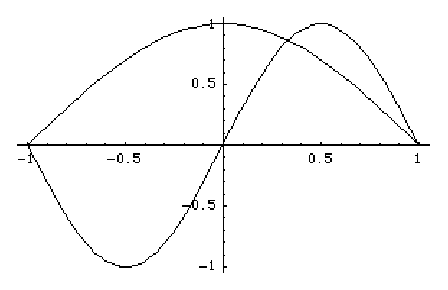
\includegraphics[scale=0.7]{wavefun1}
\end{figure}

The most probable values for position can be obtained from the squared wavefunctions:

\begin{figure}[htp!]
\centering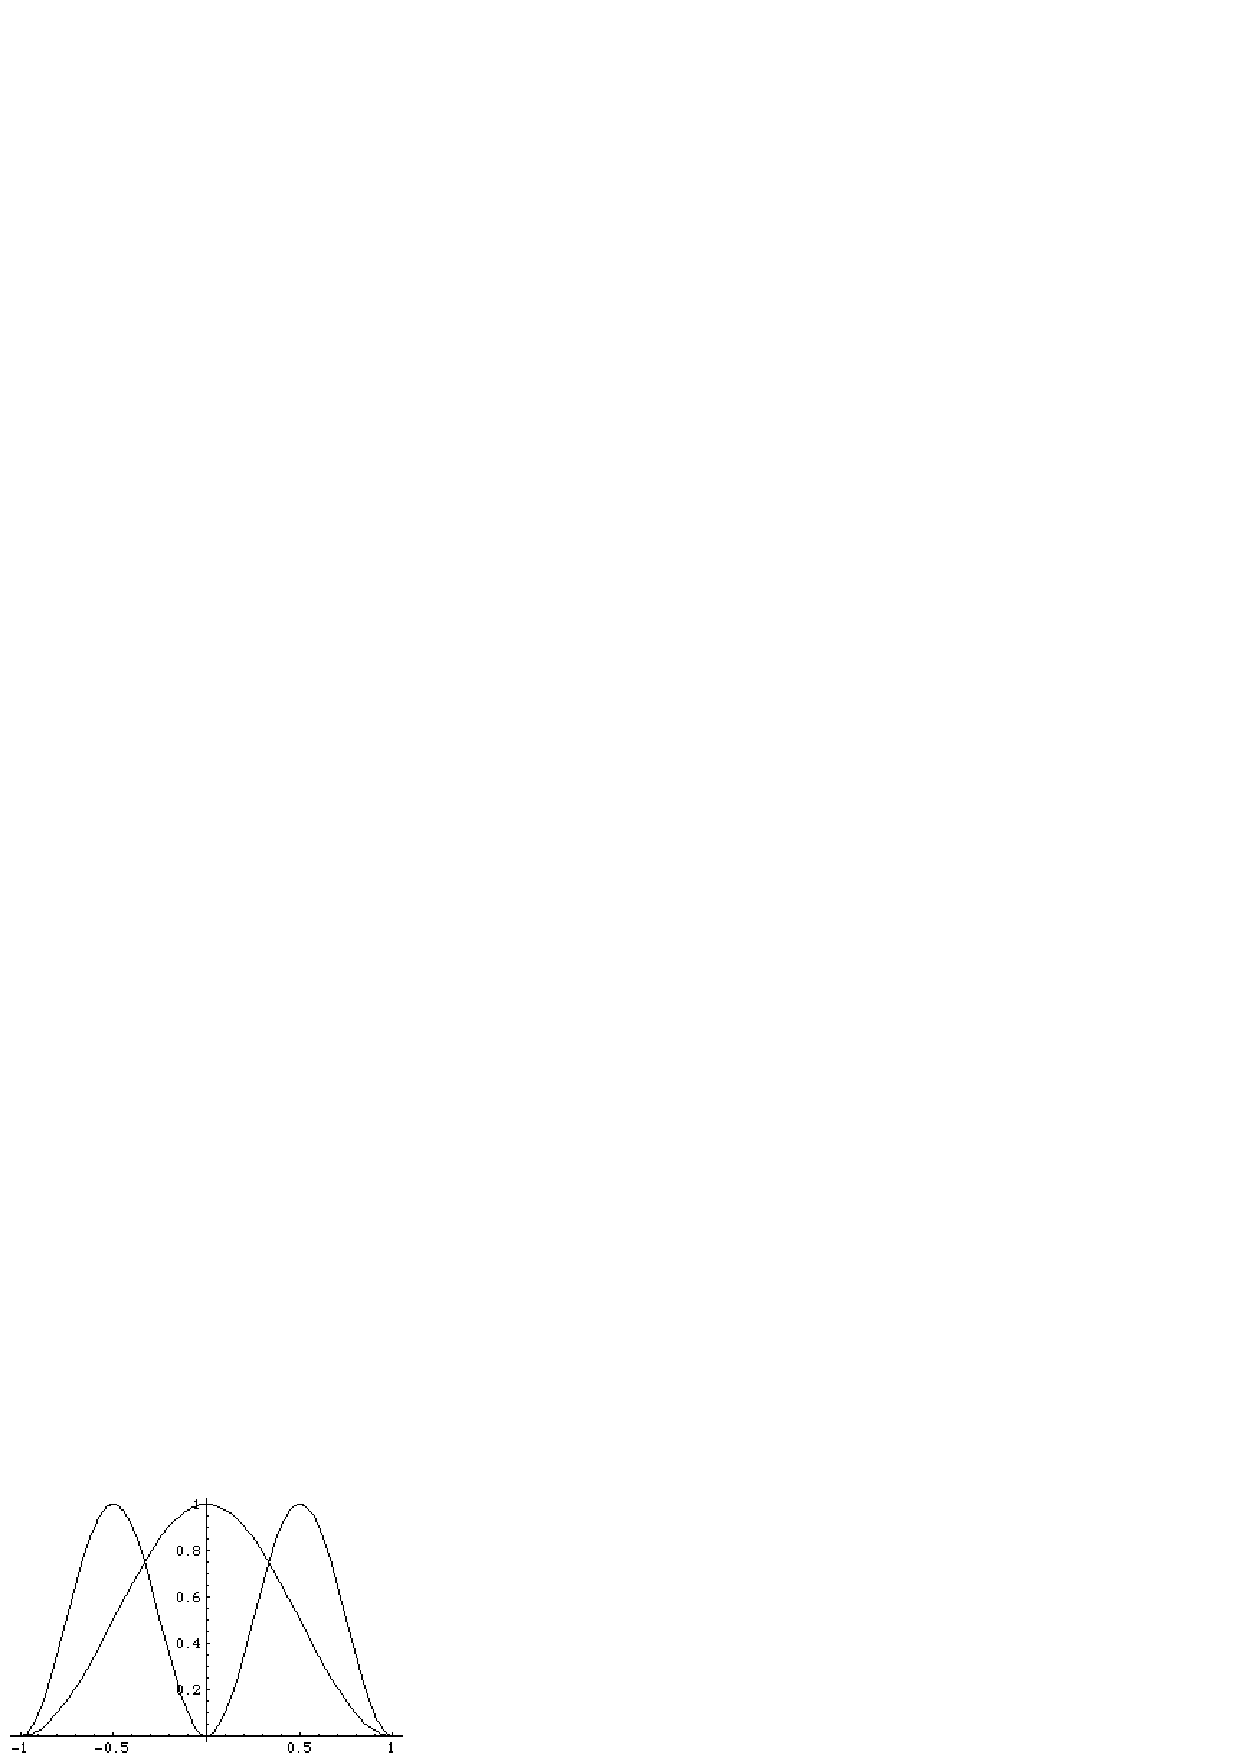
\includegraphics[scale=0.7]{wavefun2}
\end{figure}

$\psi_1$ has the maximum value at $r = 0$ whereas $\psi_2$ has two maxima at $\pm 0.5$. Note that on average both will give an outcome of $\left<\hat{r}\right> = 0$.

\item The most probable positions are given by the square of the wavefunction $\psi_0(x) = \left(2/L\right)^{1/2}\sin(3\pi x/L)$. The probability function is then $\left|\psi_0(x)\right|^2 \propto \sin^2(3\pi x/L)$. The extremum points for this function can be obtained by:
\begin{eqnarray}
\nonumber
& & \frac{d}{dx}\left(\sin^2(3\pi x/L)\right) = 0 \Rightarrow \sin(3\pi x/L)\cos(3\pi x/L) = 0\\
\nonumber
& & \Rightarrow \frac{3\pi x}{L} = n\pi\textnormal{ or }\frac{3\pi x}{L} = \left(n + \frac{1}{2}\right)\pi\\
\nonumber
& & \Rightarrow x = \frac{n}{3}L\textnormal{ or }x = \frac{n + 1/2}{3}L
\end{eqnarray}

Second derivatives can be used to identify the extrema:

$$\frac{d^2}{dx^2}\left(\sin^2(3\pi x/L)\right) \propto \cos^2\left(\frac{3\pi x}{L}\right) - \sin^2\left(\frac{3\pi x}{L}\right)$$

At $x = \frac{n}{3}L$ the values are positive which means that these correspond to (local) minima. For $x = \frac{n+1/2}{3}L$ the values are negative
and these points correspond to (local) maxima. For example, when $L = 2$ the probability function looks like:

\begin{figure}[htp!]
\centering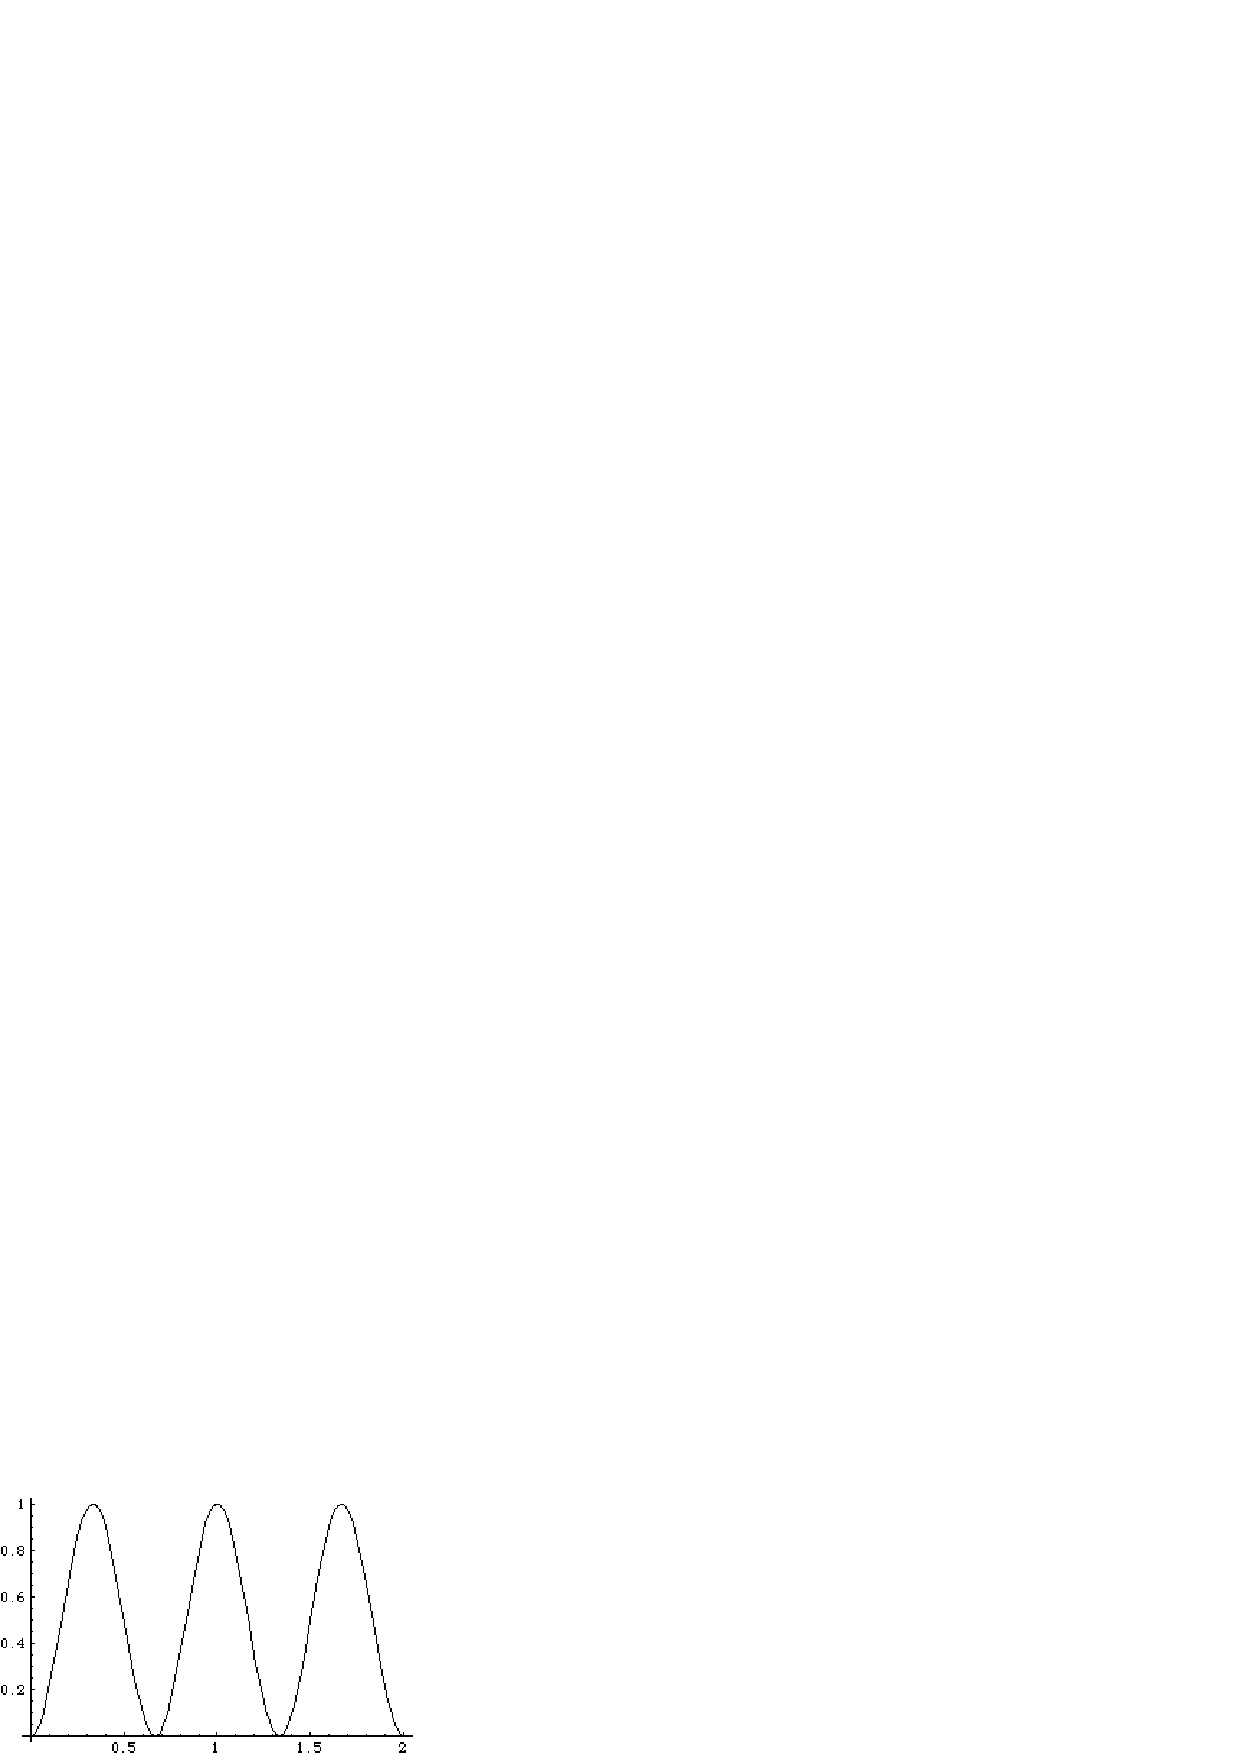
\includegraphics[scale=0.7]{wavefun3}
\end{figure}

\end{enumerate}

\hrule\vspace{0.5cm}
}{}

\item Calculate the uncertainty product $\Delta p\Delta x$ for the following wavefunctions:

\begin{enumerate}
\item $\psi_n(x) = \left(\frac{2}{a}\right)^{1/2}\sin\left(\frac{n\pi x}{a}\right)\textnormal{ with }0\le x\le L\textnormal{ (particle in a box)}$
\item $\psi_n(x) = N_vH_v\left(\sqrt{\alpha}x\right)\exp\left(-\frac{\alpha x^2}{2}\right)\textnormal{ (harmonic oscillator)}$
\end{enumerate}

\ifthenelse{\equal{\solutions}{true}}{% Problem 6/1 solution
\noindent
\underline{Solution:}\\

The equations in the lecture notes can be rewritten as (the definition of critical point and the equation of state):

$$\frac{RT_c}{\left(\bar{V}_c - b\right)^2} = \frac{2a}{\bar{V}_c^3}$$
$$\frac{2RT_c}{\left(\bar{V}_c - b\right)^3} = \frac{6a}{\bar{V}_c^4}$$
$$P_c = \frac{RT_c}{\bar{V}_c - b} - \frac{a}{\bar{V}_c^2}$$

Division of the first equation by the second (side by side) yields $\bar{V}_c = 3b$. Substitution of this expression into the first equation above gives $T_c = \frac{8a}{27Rb}$. Substitution of the two previous equations into the last equation above yields $P_c = 
\frac{a}{27b^2}$. Note that the van der Waals constants $a$ and $b$ are usually calculated using the critical temperature and pressure since they are typically known more accurately than the critical volume.

\hrule\vspace{0.5cm}
}{}

\item Scanning tunneling microscopy (STM) is a technique for visualizing samples at atomic resolution. It is based on tunneling of electron through the vacuum space between the STM tip and the sample. The tunneling current ($I\propto \left|\psi\right|^2$ where $\psi$ is the electron wavefunction) is very sensitive to the distance between the tip and the sample. Assume that the wavefunction for electron tunneling through the vacuum is given by $\psi(x) = B\exp^{-Kx}$ with $K = \sqrt{2m_e(V - E)/\hbar^2}$ and $V - E =$ 2.0 eV. What would be the relative change in the tunneling current $I$ when the STM tip is moved from $x_1 = 0.50$ nm to $x_2 = 0.60$ nm from the sample (e.g. $I_1 / I_2 =$ ?).

\ifthenelse{\equal{\solutions}{true}}{% Problem 7/1 solution
\noindent
\underline{Solution:}\\

The current is proportional to the square the wavefunction ($\left|\psi(x)\right|^2$):
\begin{eqnarray}
\nonumber
& & I\propto \left|\psi(x)\right|^2 = B^2e^{-2Kx}\\
\nonumber
& & \frac{I_1}{I_2} = e^{-2K(x_1 - x_2)}\\
\nonumber
& & K=\left(2m_e\underbrace{(V - E)}_{=2\textnormal{ eV}}/\hbar^2\right)^{1/2}\\
\nonumber
& & = \left(\frac{2(9.11\times 10^{-31}\textnormal{ kg})(2.0\textnormal{ eV})(1.602\times 10^{-19}\textnormal{J/eV})}{(1.0546\times 10^{-34}\textnormal{ Js})^2}\right)^{1/2}\\
\nonumber
& & -2K(x_1 - x_2) = -2K\times(0.10\times 10^{-9}\textnormal{ m}) \approx 1.45\\
\nonumber
& & \Rightarrow \frac{I_1}{I_2} \approx 4.3
\end{eqnarray}

\hrule\vspace{0.5cm}
}{}

\item Show that the sperhical harmonic functions a) $Y_{0,0}$, b) $Y_{2,-1}$ and c) $Y_{3,3}$ are eigenfunctions of the (three-dimensional) rigid rotor Hamiltonian. What are the rotation energies and angular momenta in each case?

\ifthenelse{\equal{\solutions}{true}}{% Problem 8/1 solution
\noindent
\underline{Solution:}\\
\begin{eqnarray}
\nonumber
& & \hat{H}\psi(r,\theta,\phi) = E\psi(r,\theta,\phi)\textnormal{ where }\hat{H}=-\frac{\hbar^2}{2I}\Lambda^2\\
\nonumber
& & \Lambda^2 = \frac{1}{\sin^2(\theta)}\frac{\partial^2}{\partial\phi^2} + \frac{1}{\sin(\theta)}\frac{\partial}{\partial\theta}\sin(\theta)\frac{\partial}{\partial\theta}
\end{eqnarray}

Since $-\frac{\hbar^2}{2I}$ is constant, it is sufficient to show that spherical harmonics are eigenfunctions of $\Lambda^2$. We operate on the given spherical harmonics by $\Lambda^2$.
\begin{enumerate}
\item $\Lambda^2Y_0^0(\theta,\phi) = \Lambda^2\frac{1}{2\sqrt{\pi}} = 0\textnormal{ (no angular dependency)}$. The rotation energy is $E = -\frac{\hbar^2}{2I}\times 0 = 0$. Also $L^2 = 0\times\hbar^2 \Rightarrow L = 0$ (since $\hat{L}^2 = -\hbar^2\Lambda^2$).
\item $\Lambda^2Y_2^{-1}(\theta,\phi) = \textnormal{ ...differentiation...} = -6Y_2^{-1}(\theta,\phi)$. The rotation energy is $E = -\frac{\hbar^2}{2I}\times (-6) = \frac{3\hbar^2}{I}$. Also $L^2 = 6\times\hbar^2 \Rightarrow L = \sqrt{6}\hbar$.
\item Expression for $Y_3^3$ was not given in the lecture notes. We use Maxima to obtain the expression: $Y_3^3(\theta,\phi) = \frac{5\sqrt{7}e^{3\phi i}\sin^3(\theta)}{8\sqrt{5\pi}}$. Then we need to evaluate: $\Lambda^2Y_3^3(\theta,\phi) = \textnormal{ ...differentiation...} = -12Y_3^3(\theta,\phi)$.
From this we can get the rotational energy as $E = \frac{6\hbar^2}{I}$. Also $L^2 = 12\times\hbar^2 \Rightarrow L = \sqrt{12}\hbar$.
\end{enumerate}

\hrule\vspace{0.5cm}
}{}

\item Calculate the z-component of angular momentum and the rotational kinetic energy in planar (e.g. 2-dimensional; rotation in $xy$-plane) rotation for the following wavefunctions ($\phi$ is the rotation angle with values between $\left[0, 2\pi\right[$):

\begin{enumerate}
\item $\psi = e^{i\phi}$
\item $\psi = e^{-2i\phi}$
\item $\psi = \cos(\phi)$
\item $\psi = \cos(\chi)e^{i\phi} + \sin(\chi)e^{i\phi}$
\end{enumerate}

\ifthenelse{\equal{\solutions}{true}}{% Problem 9/1 solution
\noindent
\underline{Solution:}\\

The Hamiltonian for 2-D rotation is $\hat{H} = \frac{\hat{L}_z^2}{2I} = -\frac{\hbar^2}{2I}\frac{d^2}{d\phi^2}$ where the rotation axis is denoted by $z$ and $\phi$ is the angle of rotation.

\begin{enumerate}
\item Operate first by $\hat{L}_z$ on $e^{i\phi}$: $\hat{L}_ze^{i\phi} = -i\hbar\frac{d}{d\phi}e^{i\phi} = \hbar e^{i\phi}$. Thus $\hat{H}e^{i\phi} = \frac{\hbar^2}{2I}e^{i\phi}$.
\item The same reasoning gives: $\hat{L}_z e^{-2i\phi} = -i\hbar\frac{d}{d\phi}e^{-2i\phi} = -2\hbar e^{-2i\phi}$ and $\hat{H}e^{-2i\phi} = \frac{4\hbar^2}{2I}e^{-2i\phi}$.
\item The given wavefunction is not an eigenfunction of $\hat{L}_z$: $\hat{L}_z\cos(\phi) = -i\hbar\left(-\sin(\phi)\right)$ (expectation value is zero).
However, it is an eigenfunction of $\hat{H}$: $\hat{H}\cos(\phi) = -\frac{\hbar^2}{2I}\frac{d^2}{d\phi^2}\cos(\phi) = \frac{\hbar^2}{2I}\cos(\phi)$.
\item Operation by $\hat{L}_z$ would change the plus sign in the middle of the wavefunction into a minus, hence this is not an eigenfunction of $\hat{L}_z$. It is an eigenfunction of $\hat{H}$: $\hat{H}(\cos(\chi)e^{i\phi} + \sin(\chi)e^{-i\phi}) = -\frac{\hbar^2}{2I}\left((i)^2\cos(\chi)e^{i\phi} + (-i)^2\sin(\chi)e^{-i\phi}\right) = \frac{\hbar^2}{2I}\left(\cos(\chi)e^{i\phi} + \sin(\chi)e^{-i\phi}\right)$.
\end{enumerate}

\hrule\vspace{0.5cm}
}{}

\end{enumerate}
